\documentclass{beamer}
  \usepackage[english]{babel}
  \usepackage[utf8]{inputenc}
  \usepackage{times}
  \usepackage{amsmath,amsthm, amssymb, latexsym,ragged2e}
  \boldmath
  \usepackage{multicol}
  
  \usetheme{Poster}
  \usepackage[orientation=portrait,size=a0,scale=1.4]{beamerposter}



% Abstract

% Nous implémentons un modèle de développement d'un organisme de type slime mould, qui a été introduit en biologie, et l'appliquons à la conception des réseaux de transport. À partir d'un réseau potentiel couvrant l'espace et d'une distribution d'origines et destinations, l'algorithme renforce itérativement les liens les plus fréquentés, pour converger vers un réseau auto-organisé adapté à la distribution des trajectoires de mobilité. Son application est illustrée pour la conception d'un réseau de ligne de bus et d'un réseau routier, sur des cas d'étude réels. Nous démontrons par ailleurs la capacité du modèle à générer un ensemble de réseaux optimaux au sens de Pareto pour les deux objectifs contradictoires de robustesse et de coût, par une exploration systématique par l'intermédiaire du logiciel OpenMOLE, sur un système métropolitain polycentrique stylisé



  \title[Beamer Poster]{Des systèmes naturels aux systèmes urbains: génération de réseaux de transport optimaux par modèle \emph{slime-mould}}
  \author[juste.raimbault@polytechnique.edu]{J. Raimbault$^{1,2}$}
  \institute[]
  {$^1$ UPS CNRS 3611 ISC-PIF et $^2$ UMR CNRS 8504 Géographie-cités\vspace{1cm}}
  \date{}
  
  \logo{
  \hfill
  
\includegraphics[height=8cm,width=0.65\columnwidth]{figures/isc}
  
\includegraphics[height=8cm,width=0.29\columnwidth]{figures/geocite}
  \hfill\hfill
  }


  %%%%%%%%%%%%%%%%%%%%%%%%%%%%%%%%%%%%%%%%%%%%%%%%%%%%%%%%%%%%%%%%%%%%%%%%%%%%%%%%%5
  \begin{document}
  \begin{frame}{} 
  
    \vfill
    \begin{columns}[t]
      \begin{column}{.49\textwidth}
      
      \vspace{-1cm}
      
        \begin{block}{Introduction}
        \vspace{-1cm}
        \begin{columns}[t]
        \begin{column}{.95\textwidth}
          \begin{itemize}         
          \item \begin{justify}%Conception et évaluation des infrastructures de transport généralement \emph{top-down} (approche type modèles d'interaction transport-usage du sol~\cite{wegener2004land}).
          Méthodes classiques de conception et d'évaluation des infrastructures de transport basée sur scenarios exogènes \cite{wegener2004land}; optimisation et/ou analyse de données.
          \end{justify}
          \bigskip
          %Récente introduction des méthodes de \emph{bio-mimétisme} pour le design et le management des systèmes technico-sociaux complexes~\cite{doursat2012morphogenetic}.
          \item \begin{justify} Ingénierie morphogénétique à la croisée des systèmes auto-organisés et architecturés \cite{doursat2012morphogenetic}: application démontrée à la conception d'infrastructures de transports~\cite{bebber2007biological}.
          \end{justify}
          %\bigskip
          %\item Application démontrée à la conception d'infrastructures de transports~\cite{bebber2007biological}. %  par optimisation multi-objectif (ex. coût, robustesse) émergente
          \bigskip
          \item \begin{justify}Application d'un modèle de croissance de \emph{slime-mould} à la conception multi-objectifs d'un réseau de transport.\end{justify}
          \end{itemize}
          \end{column}
          \end{columns}
        \end{block}
        
         \begin{block}{Modèle}
        %\vspace{-1cm}
        \begin{columns}[t]
        \begin{column}{.95\textwidth}
        \vspace{-2cm}
        \begin{justify}
          Modèle de croissance d'un \emph{slime-mould}~\cite{tero2010rules} : principe \emph{d'exploration puis renforcement}.
          %pour une moisissure à la recherche de ressources.
          
          \bigskip
          
          Etude de l'aspect renforcement : réseau initial homogène de tubes $ij$, longueur $L_{ij}$, diamètre variable $D_{ij}$, traversés par un flux de fluide $Q_{ij}$. Sommets $i$ à la pression $p_i$. Un nombre de noeuds $N$ sont à desservir, parmi eux aléatoirement à chaque étape l'un est source $p_{i_+}=I_0$ et l'autre puits $p_{i_-}=-I_0$
          
          
          \bigskip
          \textit{Itération du modèle :}
          \begin{enumerate}
          \item Détermination des flux par lois de Kirchoff (analogie électrostatique, résolution d'un système fermé) : loi d'Ohm
          \begin{equation}
Q_{ij}=\frac{D_{ij}}{L_{ij}}\cdot(p_{i}-p_{j})
\end{equation}
et conservation des flux
\begin{equation}
\sum_{j\rightarrow i}Q_{ij} = 0 , \sum_{j\rightarrow i_\pm}Q_{i_{\pm}j} = \pm I_0
\end{equation}



\item Evolution du diamètres de tubes ($\gamma$ paramètre de renforcement)
\begin{equation}
\frac{dD_{ij}}{dt}=\frac{\left|Q_{ij}\right|^{\gamma}}{1+\left|Q_{ij}\right|^{\gamma}}-D_{ij}
\end{equation}
          \end{enumerate}

\bigskip

Extraction du réseau final après convergence selon un paramètre de seuil de diamètre ou un nombre maximal d'itérations.
 %(distributions finales généralement bimodales).

%\bigskip 
%\textit{Modèle multi-échelle :} Dynamique des diamètres supposées constantes pendant l'itération pour obtenir les flux. 
%\bigskip 
%\textit{Implémentation en NetLogo ouverte~\cite{impl}}

\end{justify}
          \end{column}
          \end{columns}
        \end{block}
        
        
        \begin{block}{Indicateurs}
       \vspace{-2cm}
        \begin{columns}[t]
        \begin{column}{.95\textwidth}
        \begin{justify}
          Comportement du modèle évalué au travers d'indicateurs contradictoires de performance pour le réseau généré :
          %$(V_f,E_f)$, qui peuvent être vu comme des objectifs contradictoires :
          \bigskip
          \begin{itemize}
          \item Coût de construction $c=\sum_{ij\in E_f}D_{ij}(t_f)$
          \bigskip
          \item \begin{justify}Performance moyenne~\cite{banos2012towards}
          \[
          v=\frac{1}{|V_f|^2}\sum_{i,j\in V_f}\frac{d_{i\rightarrow j}}{||\vec{i}-\vec{j}||}
          \]
          \end{justify}
          \bigskip
          \item Robustesse (indice \textit{Network Trip Robustness}, impact de la suppression des liens~\cite{sullivan2010identifying})
          \end{itemize}

          \end{justify}
          \end{column}
          \end{columns}
        \end{block}
        
        \begin{block}{Exploration du modèle}
        \begin{columns}[t]
        \begin{column}{.7\textwidth}
        	
        \end{column}
		\begin{column}{.25\textwidth}
        	
\includegraphics[width=\linewidth]{figures/openmole4.png}
        \end{column}
        \end{columns}
        \end{block}

        
        
%        \begin{block}{Analyse de Sensibilité}
%       \vspace{-1cm}
%        \begin{columns}[t]
%        \begin{column}{.47\textwidth}
%                    
%          \includegraphics[width=0.5\columnwidth,height=8cm]{figures/graphe_cout}
%          \includegraphics[width=0.5\columnwidth,height=8cm]{figures/graphe_NTR}\\
%          \bigskip
%          \textit{Sensibilité des indicateurs aux paramètres $(N,I_0)$.}
%          
%
%          \end{column}
%          \begin{column}{.47\textwidth}
%          
%           
%            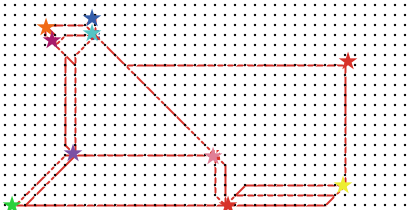
\includegraphics[width=0.5\columnwidth,height=6cm]{figures/networkDense}
%          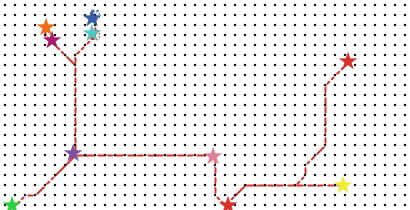
\includegraphics[width=0.5\columnwidth,height=6cm]{figures/networkLessDense}\\
%          \bigskip
%          \begin{justify}
%          \textit{Sensibilité de la topologie du réseau au coefficient de renforcement $\gamma$. Gauche : $\gamma \sim 1$, réseau robuste. Droite : $\gamma >> 1$, réseau arborescent.}
%          \end{justify}
%          \end{column}
%          \end{columns}
%        \end{block}
%        
        
      \end{column}
      
      
      \begin{column}{.49\textwidth}
      
       \begin{block}{Application : desserte optimale}
        \vspace{-1.5cm}
          \begin{columns}[t]
        \begin{column}{.95\textwidth}
        %Mission de prospective pour la mairie de Romainville : itinéraire d'une navette intra-urbaine avec points de desserte imposés.\end{justify}
       \begin{justify} Problème type voyageur de commerce, mais multi-objectif (coût, vitesse, robustesse) : itinéraire de desserte pour une navette intra-urbaine. 
       \end{justify}
         
         % la génération de réseau \emph{bottom-up} par application du modèle sur un réseau initial construit par données géographiques réelles (réseau de rues) donne une solution proche du front de Pareto.
         \bigskip\bigskip
          %\vspace{2cm}
          
          {
          \centering
          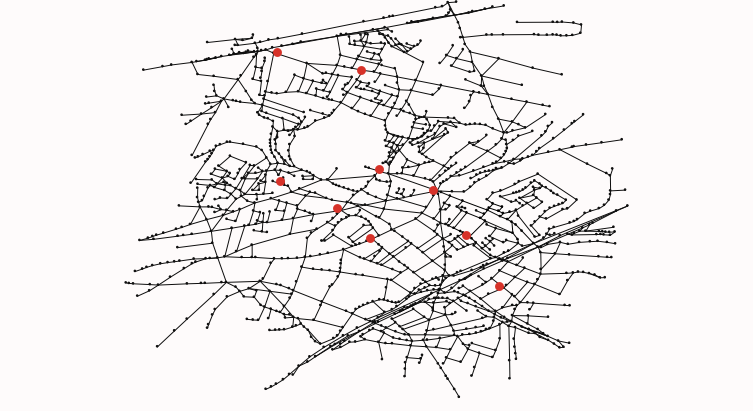
\includegraphics[width=0.32\columnwidth]{figures/tick1}
          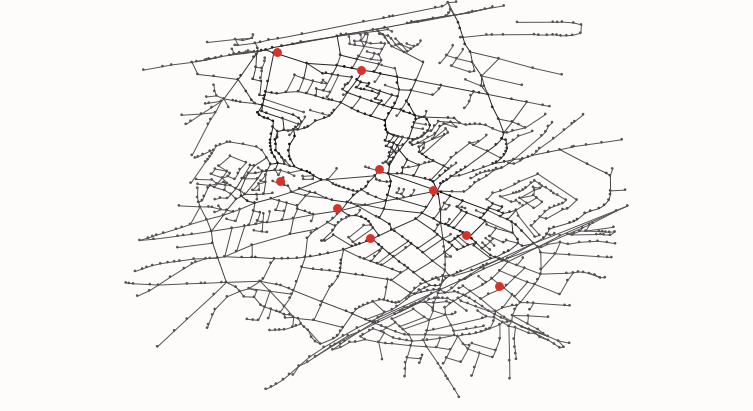
\includegraphics[width=0.32\columnwidth]{figures/tick10}
          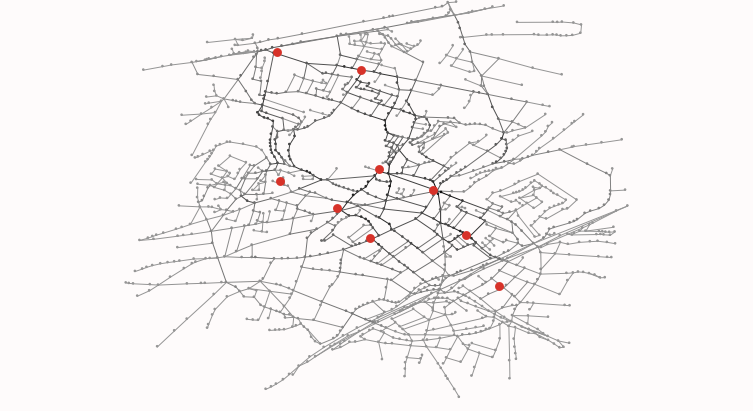
\includegraphics[width=0.32\columnwidth]{figures/tick20}\\
          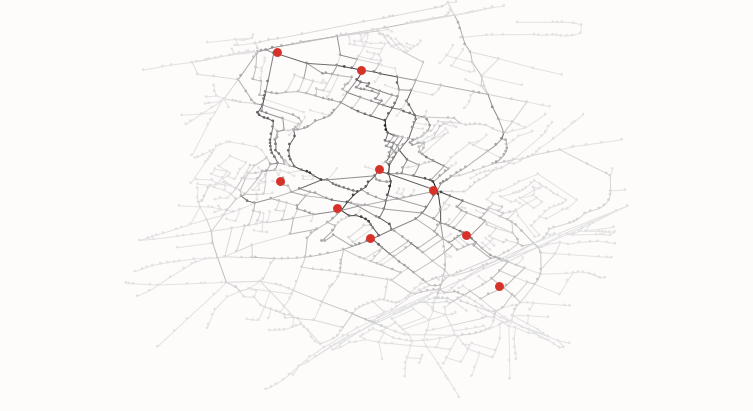
\includegraphics[width=0.32\columnwidth]{figures/tick50}
          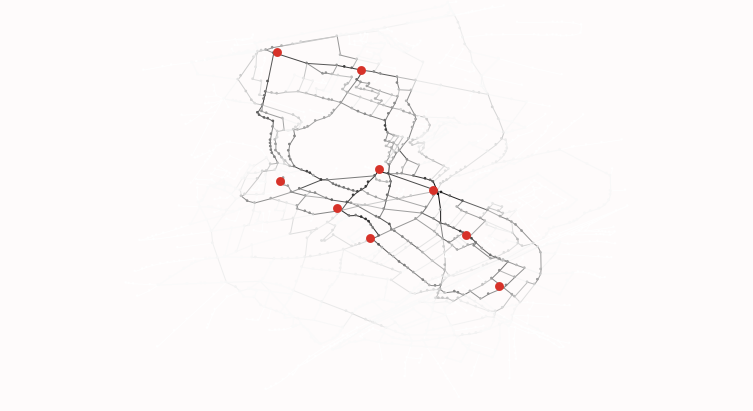
\includegraphics[width=0.32\columnwidth]{figures/tick101}
          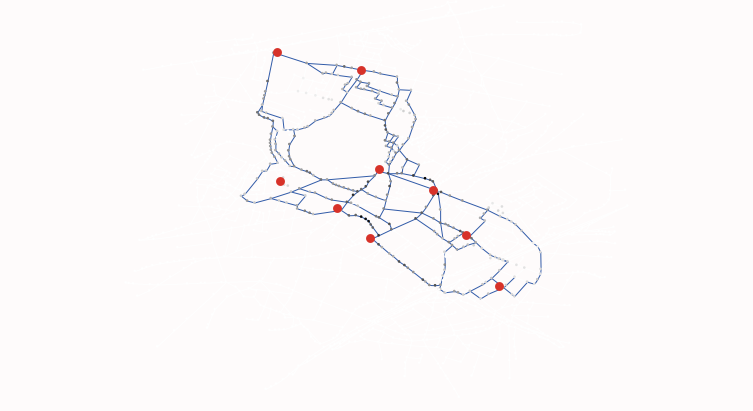
\includegraphics[width=0.32\columnwidth]{figures/reseauFinal}\\
          \bigskip
          \small\textit{Convergence progressive du réseau vers le réseau optimal desservant les points fixés (en rouge), en partant d'un réseau initial à diamètres égaux (réseau de rues).}\bigskip
          
          }
          \end{column}
          \end{columns}
        \end{block}
      
      
      
        \begin{block}{Application : réseaux métropolitains}
          \begin{columns}[t]
        \begin{column}{.95\textwidth}
        \begin{justify}
        \vspace{-2cm}
          
          %Application abstraite : \textit{étant donné une distribution de noeuds à desservir (puits), quel est le corridor optimal pour une infrastructure à plus grande échelle (ex. : réseau ferré) pour laquelle les stations sont considérées comme des sources, au sens de l'optimalité multi-critères du réseau local auto-généré dans ce contexte ?}
          
          %\bigskip
          %$\rightarrow$ Exploration heuristique d'un espace arborescent d'implantations possibles ; obtention des fronts de Pareto pour les différents indicateurs ; choix de solutions optimales au sens de Pareto
          %\vspace{1cm}
          
          Dans le cadre d'une configuration métropolitaine polycentrique stylisée \cite{le2015modeling}, comment élaborer automatiquement différents scénarios pour un nouveau réseau de transport ?
          
          \bigskip\bigskip
          
          {
          \centering
          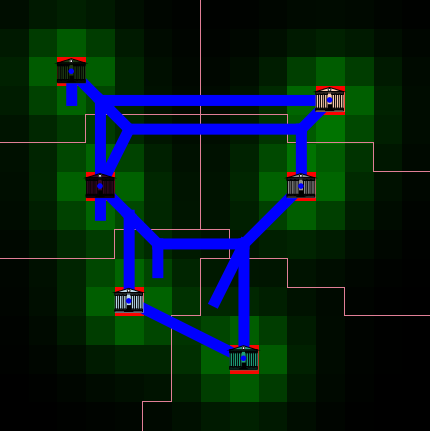
\includegraphics[width=0.33\columnwidth]{figures/bionw_territ6_gamma1_1_bis.png}
          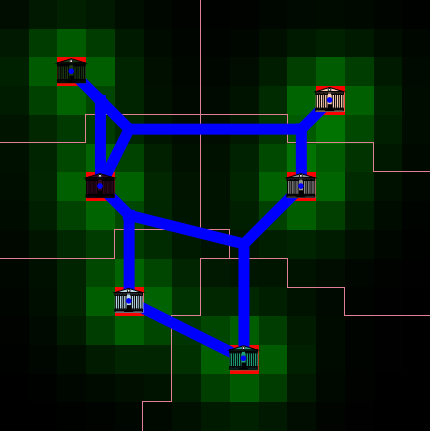
\includegraphics[width=0.33\columnwidth]{figures/bionw_territ6_gamma1_2_quart.png}
          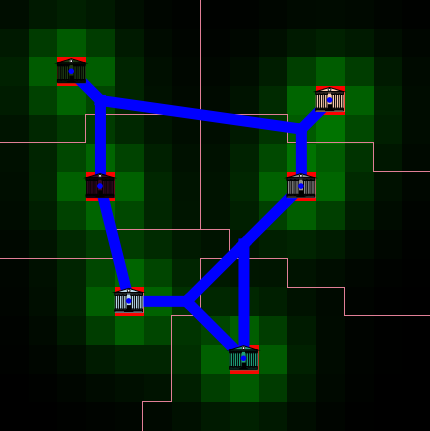
\includegraphics[width=0.33\columnwidth]{figures/bionw_territ6_gamma1_25_bis.png}\\
          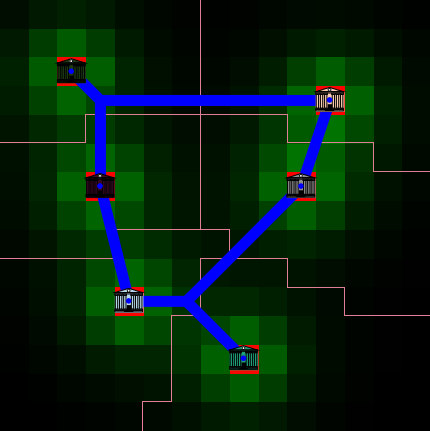
\includegraphics[width=0.33\columnwidth]{figures/bionw_territ6_gamma1_3_bis.png}
          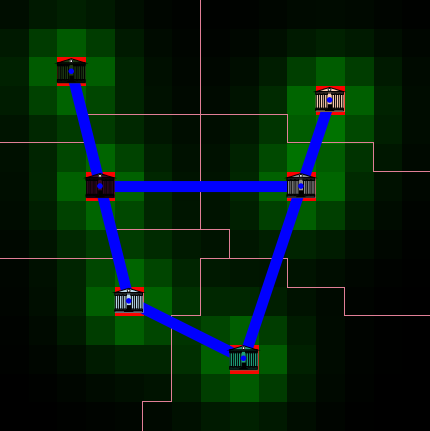
\includegraphics[width=0.33\columnwidth]{figures/bionw_territ6_gamma1_5.png}
          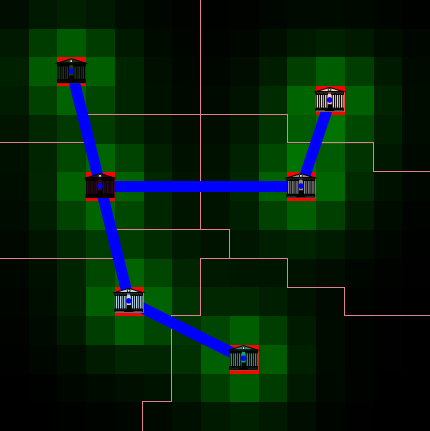
\includegraphics[width=0.33\columnwidth]{figures/bionw_territ6_gamma1_8.png}\\
          \bigskip
          \small\textit{Réseaux stylisés obtenus pour des valeurs décroissantes de $\gamma$, pour une même configuration de desserte des centres.}
          }
          
          \vspace{1.5cm}
          
          {
          \centering
          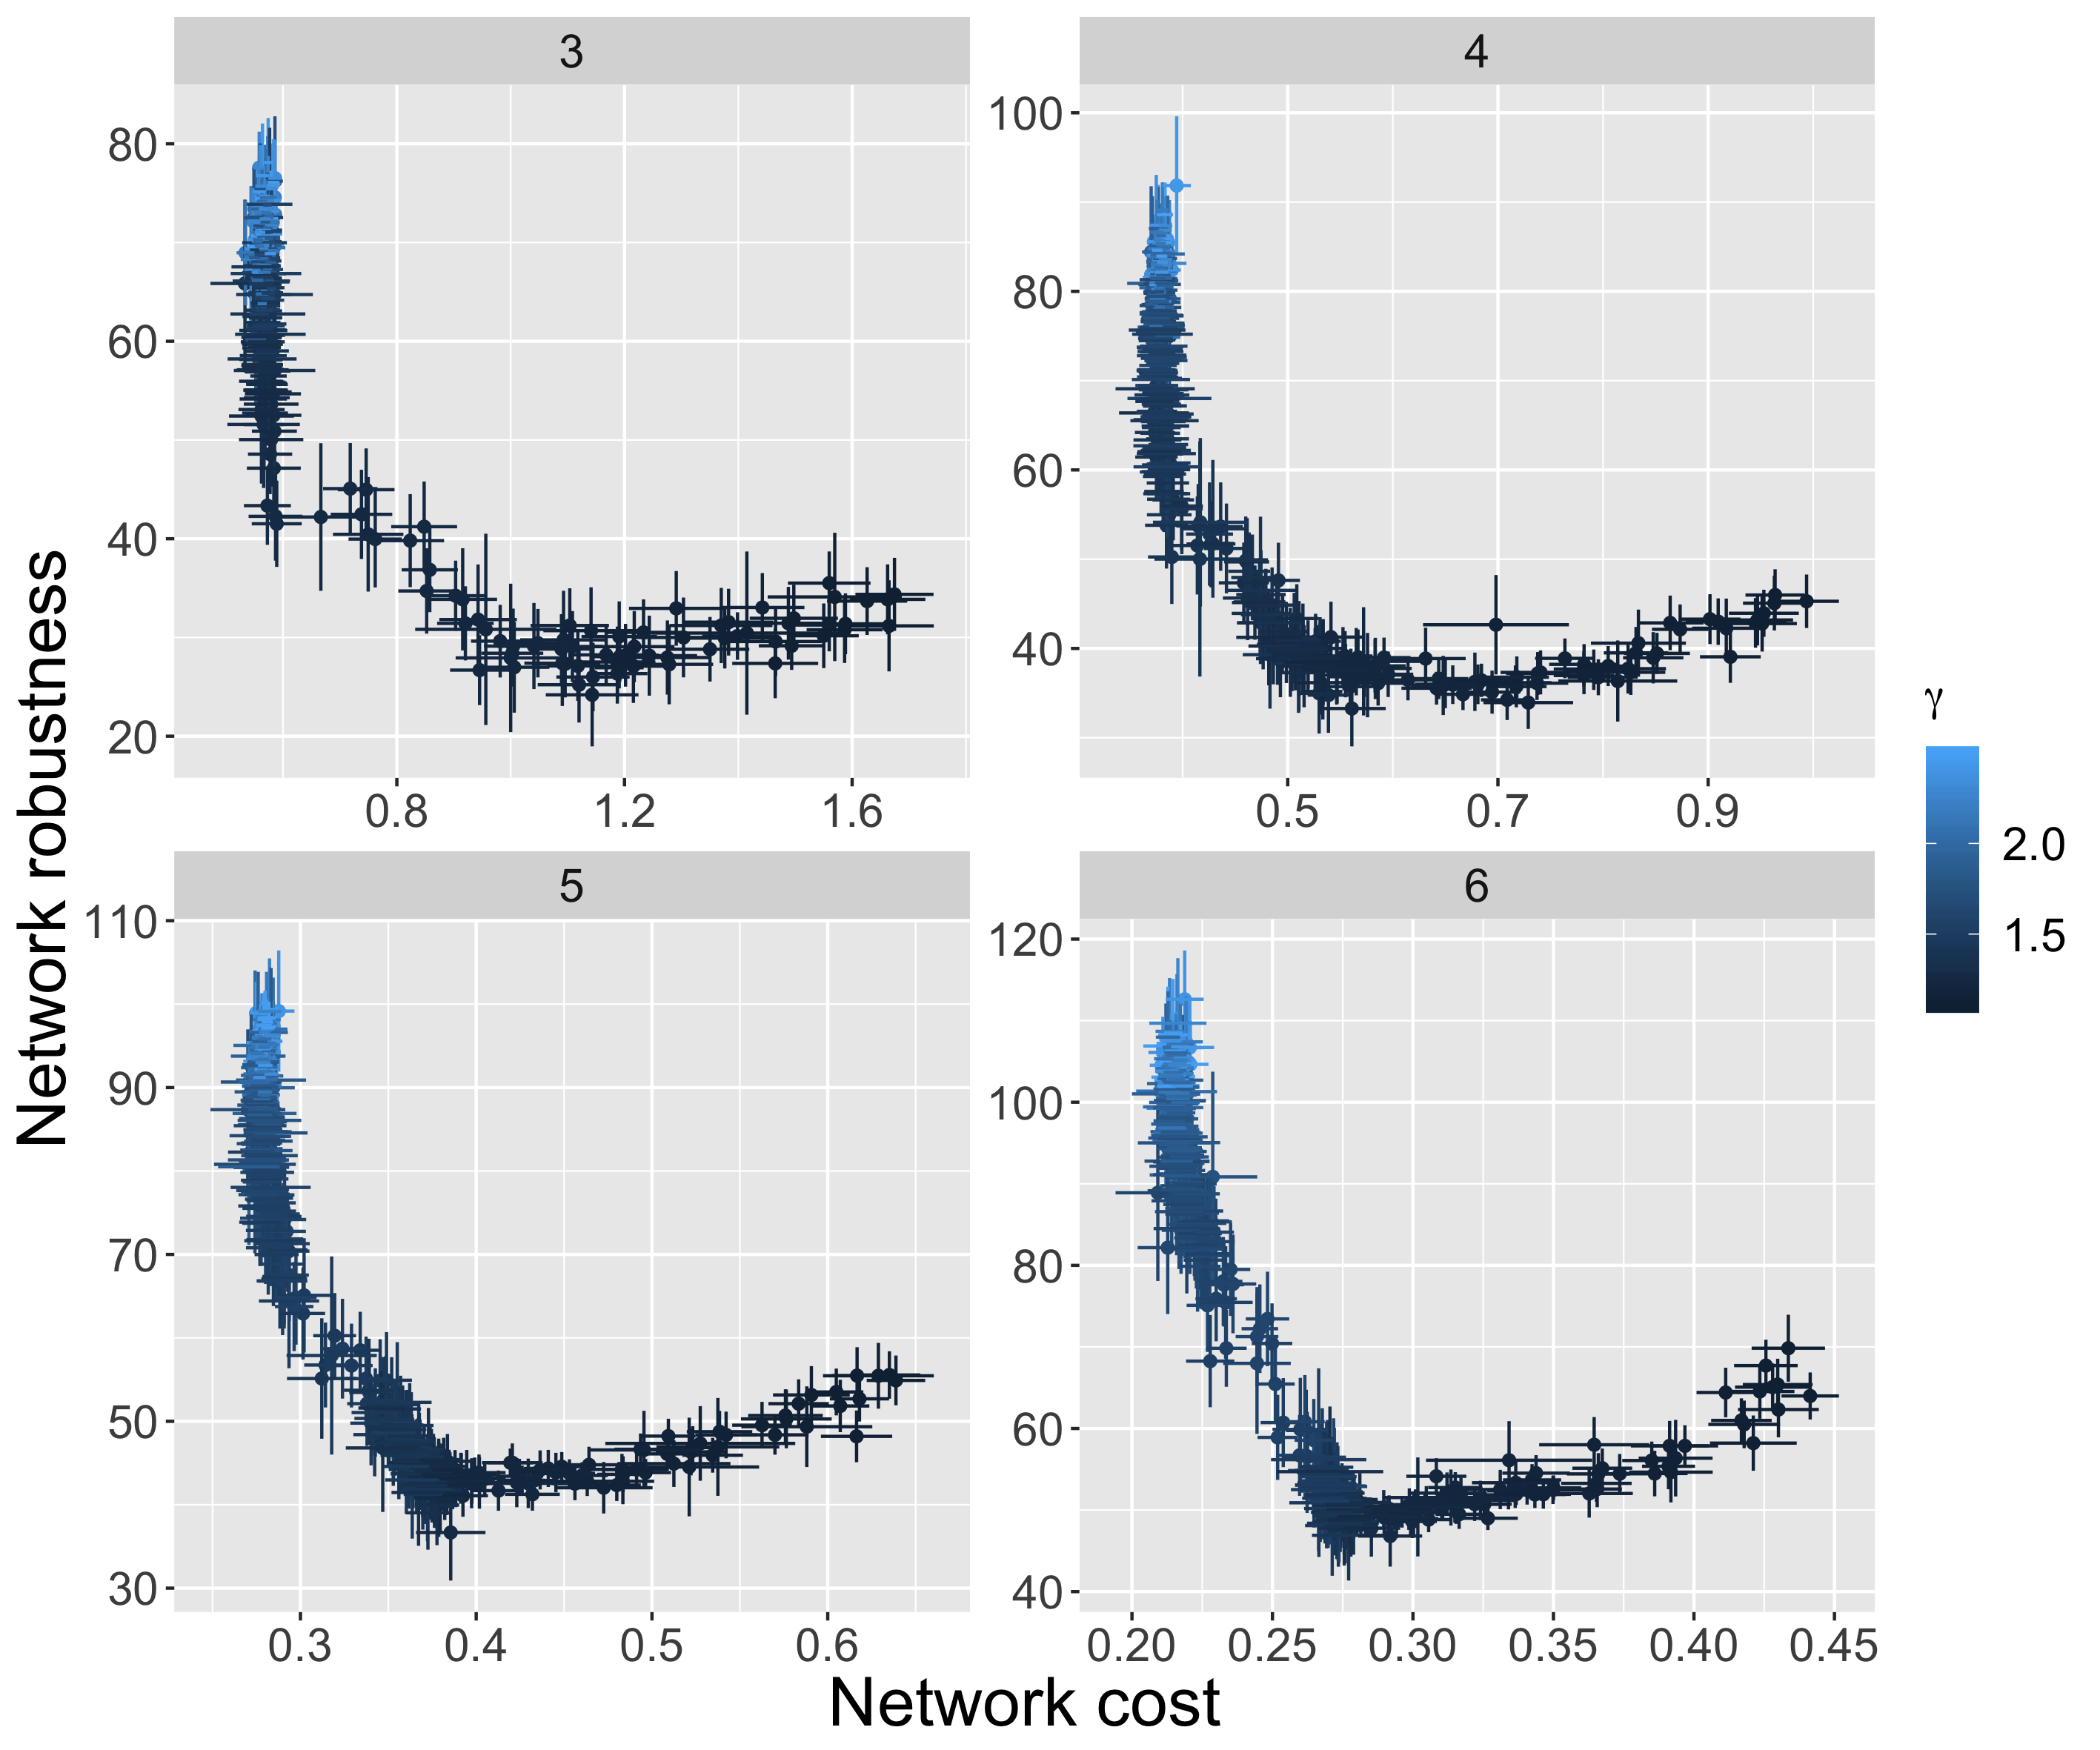
\includegraphics[width=0.49\columnwidth]{figures/pareto_cost-robustness_facetCenterNumber_withgaussianCI.png}
          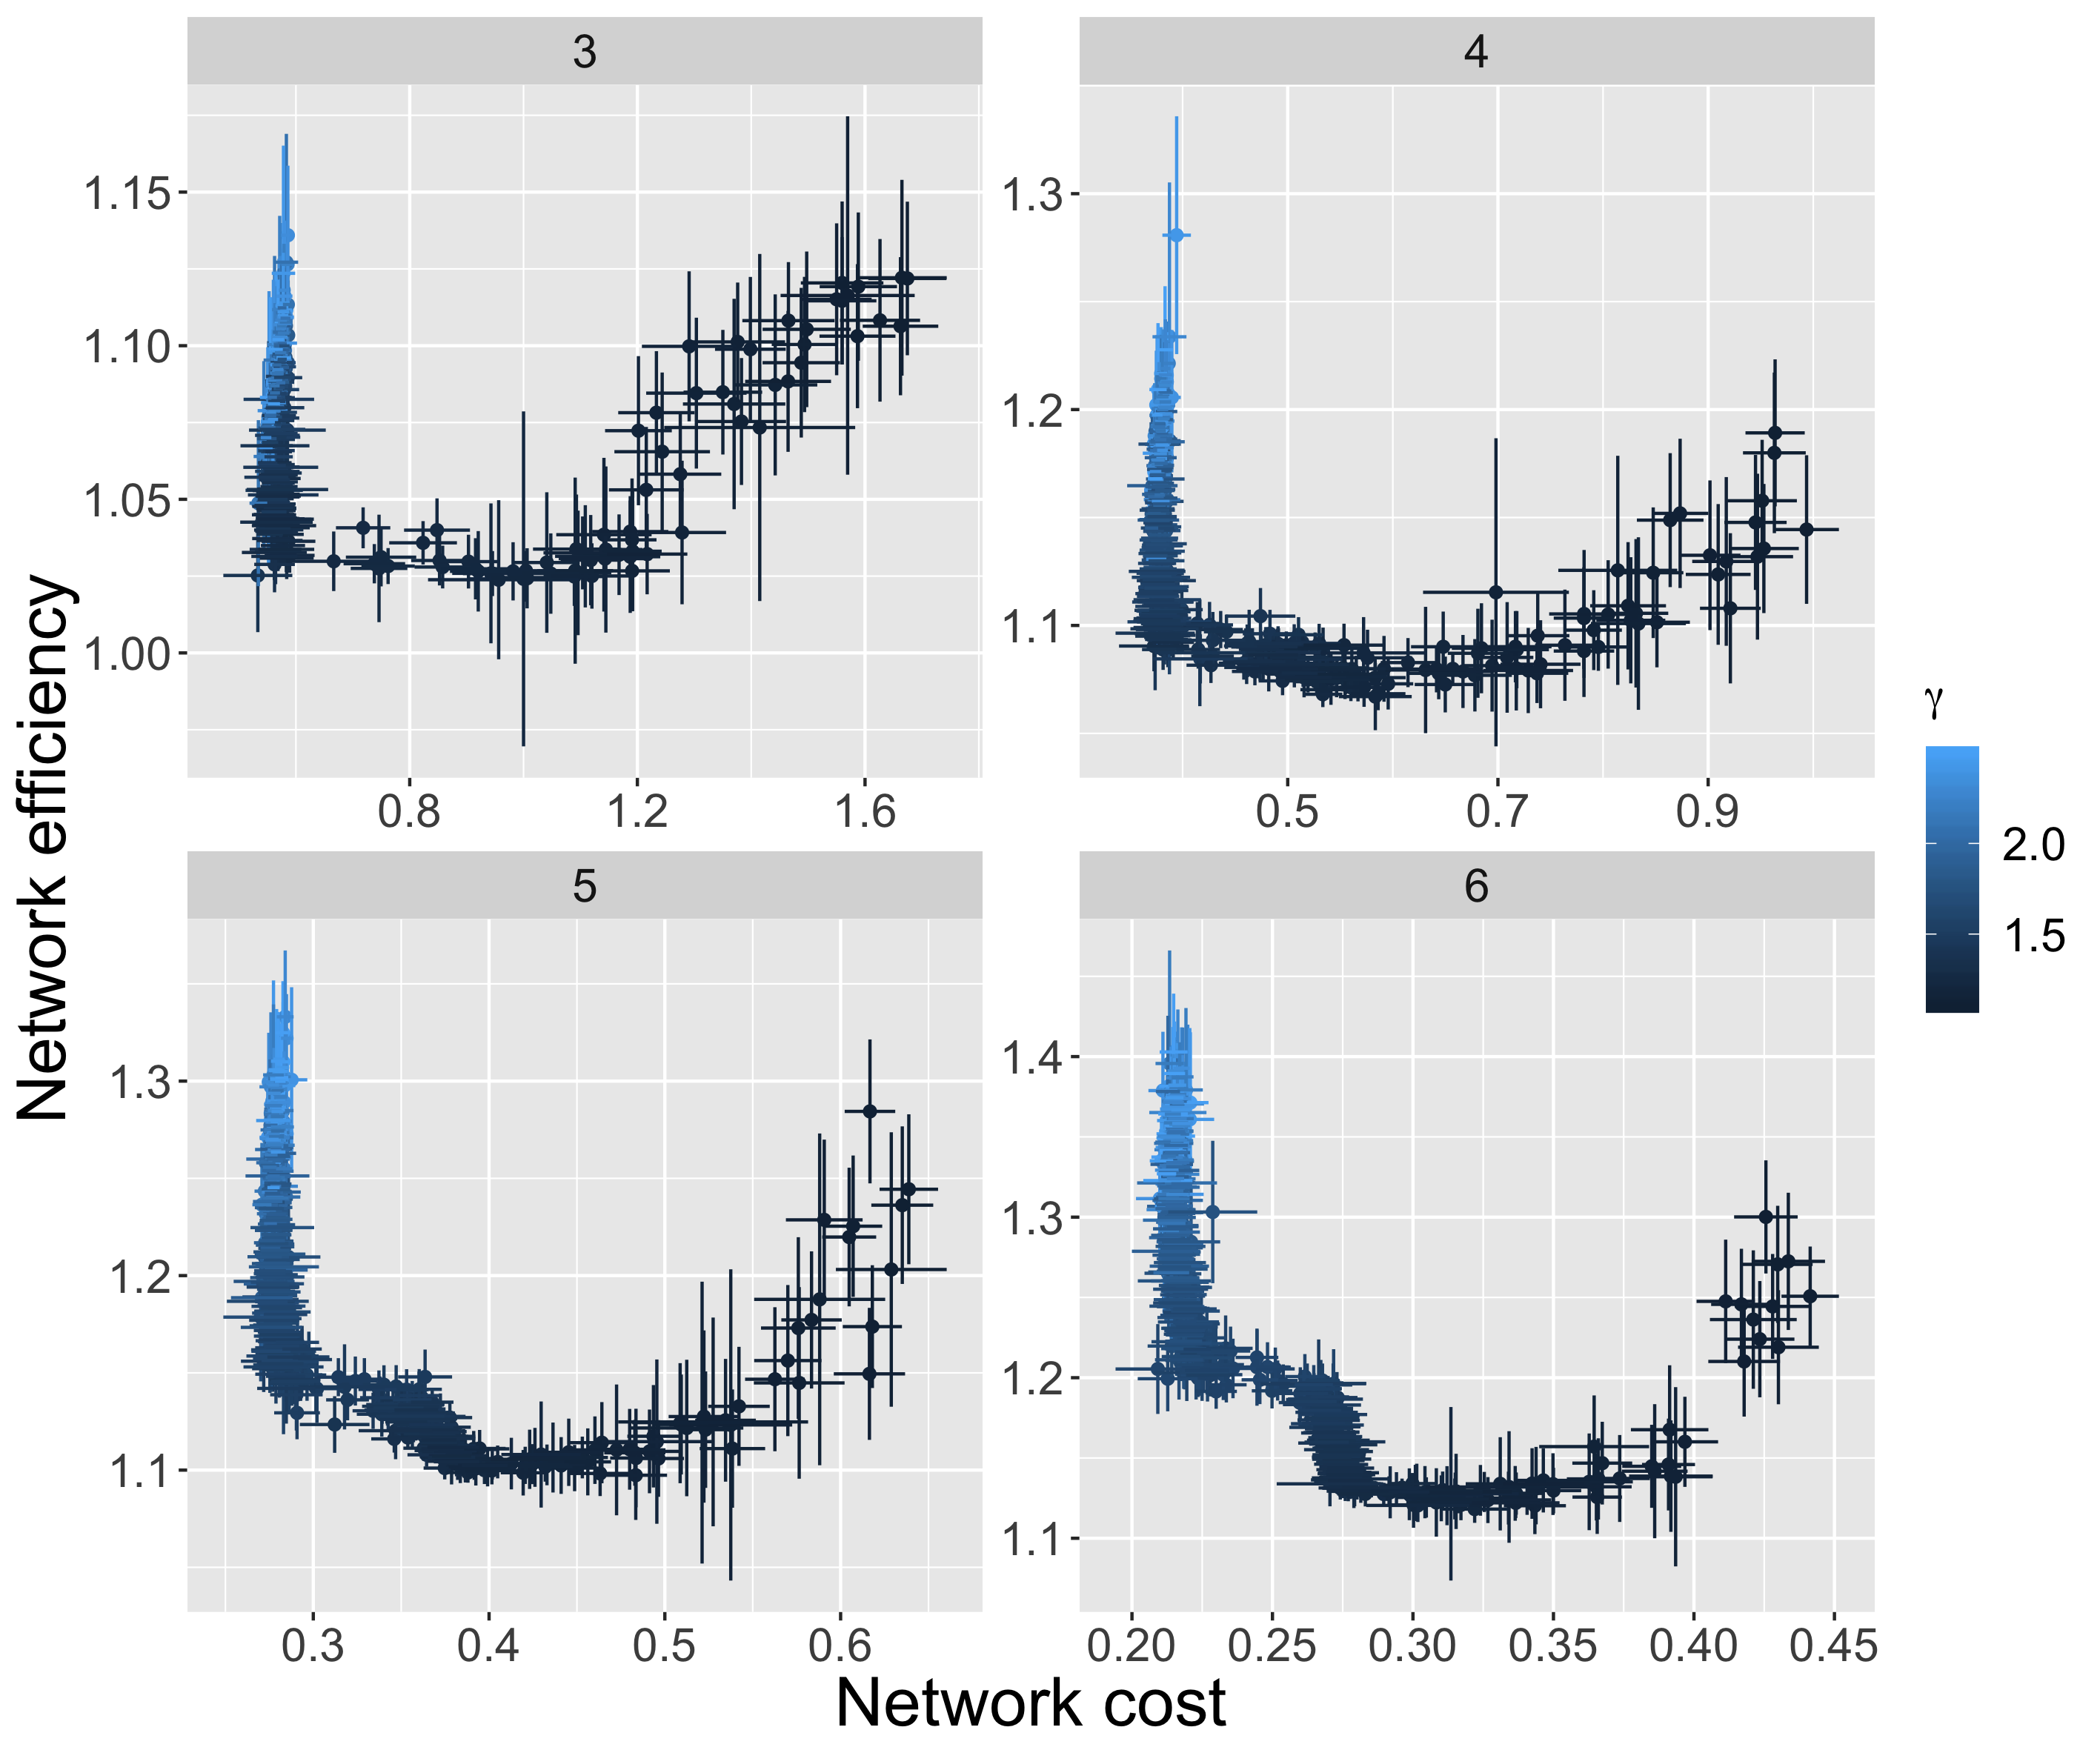
\includegraphics[width=0.49\columnwidth]{figures/pareto_cost-speed_facetCenterNumber_withgaussianCI.png}\\
         
         \bigskip
          
          \small
          \textit{Optimisation de Pareto : projection des configurations explorées dans l'espace des indicateurs, obtention du front de Pareto ; configurations correspondant à trois points optimaux.}
         }
          
          \end{justify}
          \end{column}
          \end{columns}
        \end{block}


%        \begin{block}{Conclusion}
%         \begin{columns}[t]
%        \begin{column}{.95\textwidth}
%          
%          \end{column}
%          \end{columns}
%        \end{block}
        
        
        
      \end{column}
    \end{columns}
    
    %\begin{columns}[t]
    %  \begin{column}{\linewidth}
    
    \begin{block}{References}
        {\tiny
        \vspace{-1cm}
        \begin{multicols}{4}
          \bibliographystyle{apalike}
          \bibliography{/Users/juste/ComplexSystems/CityNetwork/Biblio/Bibtex/CityNetwork,biblio}
        \end{multicols}
          }
        \end{block}
    %\end{column}
    %\end{columns}
    
  \end{frame}
\end{document}





